\documentclass{amsart}
\usepackage[foot]{amsaddr} % put addresses on first page

\usepackage{geometry}
\usepackage{booktabs}
\usepackage{graphicx,psfrag,epsf}
\usepackage{enumerate}
\usepackage{enumitem}
\usepackage{amsfonts}
\usepackage{mathtools}
\usepackage{amssymb}
\usepackage{amsmath}
\allowdisplaybreaks
\usepackage{longtable}
\usepackage{bigints}
\usepackage{siunitx}
\usepackage{algpseudocode}
\usepackage{algorithm}
\usepackage{amsthm}
\usepackage{soul}
\usepackage{color}
\usepackage{hyperref}
\usepackage[capitalise]{cleveref}
\newtheorem{theorem}{Theorem}[section]
\newtheorem{corollary}{Corollary}[theorem]
\newtheorem{lemma}{Lemma}[theorem]
\newtheorem{definition}{Definition}[section]
%

\usepackage[numbers]{natbib}
\usepackage{url} % not crucial - just used below for the URL 
\usepackage{doi}

\newcommand{\dashrule}{\hdashline\noalign{\vskip 0.5ex}}

\title{Conditional Copula models using loss-based Bayesian Additive Regression Trees}
\author{**}
\date{\today}

	\begin{document}

\begin{abstract}
	 We present a novel semi-parametric Bayesian approach for modelliing conditional copulas to understand the dependence structure between two random variables when it is influenced by a different covariate. We propose the use of Bayesian additive regression trees to model the conditional copulas. We specify a loss based prior for the BART model suggested by \citet{serafini2024lossbasedpriortreetopologies}, which is designed to reduce the loss in information and complexity for tree misspecification giving us a parsimonious model that avoids over-fitting, a common issue of BART models. We present our results with both simulated and real dataset to show the applicability and efficiency of our method.
\end{abstract}

\maketitle

\section{Introduction}

\section{Model}

\subsection{Conditional copula}

Copulas are extremely useful  for modelling the dependence structure between random variables when we wish to separate the marginals from their joint distribution. \citet{sklar:1959} showed the existence of such unique copulas $C:[0,1]^p\to [0,1]$ such that
\begin{equation*}
	H(Y_1,Y_2,\cdots, Y_p) = C(F_1(Y_1),F_2(Y_2),\cdots,F_p(Y_p)).
\end{equation*}
In some cases, there might be additional confounding random variable $X$ that influences the dependence between $Y_1,Y_2,\cdots, Y_p$. 

In such cases, a conditional copula is used to understand the dependence structure. A conditional copula was first formalised by \citet{patton2006}. For simplicity we present the formulation for two variables. Let $Y_1$ and $Y_2$ be two continuous random variables and $X$ be a continuous random variable that might affect the relationship between $Y_1$ and $Y_2$. Then according to Sklar’s theorem there exists a unique copula such that:
\begin{equation*}
	H(Y_1,Y_2\mid X) = C_X(F_{1X}(Y_1\mid X),F_{1X}(Y_2\mid X)); \quad \forall (y_1,y_2) \in \mathbb{R}^2
\end{equation*}
where $C_X \coloneqq C(\cdot\mid \theta(X))$ is the copula function that varies with respect to $X$ through the copula parameter $\theta$ and $F_{iX}(Y_i\mid X)$ is the cdf of $Y_i$ conditional on $X$ for $i=1,2$.

This gives us the following copula distribution function
\begin{equation*}
	C_X(u_1,u_2) = H\left(F_{1X}^{-1}(Y_1\mid X),F_{2X}^{-1}(Y_2\mid X)\mid X\right)
\end{equation*}
where $u_k = F_{1X}(Y_k\mid X)$ for $i=1,2$.

\subsection{Loss-based BART}

Let, $Z$ be an outcome data such that 
\begin{equation*}
	Z_i \sim \mathcal{N}\left(r(x_i),\sigma^2\right);\qquad 1\le i\le n.
\end{equation*}
Then we can approximate this function $r(x)$ with sum of regression trees such such that,
\begin{equation*}
	r(x_i) = \sum_{t=1}^m g(x_i, T_t, M_t).
\end{equation*}
where $T_t$ denotes the $t$-th tree, $M_t$ denotes the vector of terminal node values $M_t = \{\mu_1,\mu_2, \cdots, \mu_{n_L(T_t)}\}$ of the $t$-th tree and $n_L(T_t)$ denotes the number of terminal nodes of the $t$-th tree. 

Recently, \citet{serafini2024lossbasedpriortreetopologies} proposed a loss-based prior for BART in the following way:
\begin{align}
	\begin{split}
		T_t, M_t &\sim \pi(T_t)\pi(M_t\mid T_t)\\
		T_t &\propto \exp\left(\omega n_L(T_t)-\gamma\Delta(T_t)\right)\\
		\pi(M_t\mid T_t) & = \prod_{j=1}^{n_L(T_t)}\pi(\mu_j\mid T_t).
	\end{split}
\end{align}
where $\Delta(T_t)$ is the difference between right terminal nodes and left terminal nodes of $t$-th given tree.

For the choice of prior on $\mu_j\mid T_t$ \citet{chipman_BART,serafini2024lossbasedpriortreetopologies} suggested a conjugate prior with respect to the likelihood function. 

\subsection{Copula Parameter Estimation}

We wish to employ this loss-based prior for BART for the estimation of $\theta(x)$. Such that 
\begin{equation*}
	\theta(x) \coloneqq h\left(\sum_{t=1}^m g(x_i, T_t, M_t)\right).
\end{equation*}
Now, let $c\left(u_1,u_2\mid \theta(x)\right)$ denote the conditional copula density function. Then we can define the following hierarchical model
\begin{align}
	\begin{split}
		u_{1i},u_{2i} \mid \theta(x_i) & \sim c\left(u_{1i},u_{2i}\mid h\left(\sum_{t=1}^m g(x_i, T_t, M_t)\right)\right)\\
		T_t &\propto \exp\left(\omega n_L(T_t)-\gamma\Delta(T_t)\right)\\
		\pi(M_t\mid T_t) &\propto \prod_{j=1}^{n_L(T_t)}\pi(\mu_j\mid T_t)\\
		\mu_j\mid T_t &\sim \mathcal{N}(0,\sigma_{t}^2)\\
		\sigma_{t}^2&\sim \text{InvGamma}(a,b)\\
		t & = 1,2,\cdots m\\
		a,b&>0.
	\end{split}
\end{align}

This gives us the following posterior:
\begin{equation}
	\pi(T,M \mid U_1, U_2, X) \propto \prod_{i=1}^{n}c\left(u_{1i},u_{2i}\mid h\left(\sum_{t=1}^m g(x_i, T_t, M_t)\right)\right)\prod_{t=1}^{m}\pi(T_t)\prod_{t=1}^{m}\pi(M_t\mid T_t).
\end{equation}

To sample from the posterior we use backfitting algorithm where we sample $(T_j, M_j)$ conditional on the other $m-1$ pairs of $(T_k,M_k)$. Therefore, we define $R_{ij}$ such that
\begin{equation*}
	R_{ij} = \sum_{t\not=j}g(x_i, T_t, M_t)
\end{equation*}
Then the posterior of $j$-th pair conditional on $R_j$ is given by:
\begin{align}\label{eq:post:res}
	\begin{split}
		\pi(T_j,M_j \mid R_j, U_1,U_2, X) &\propto \prod_{i=1}^{n}c\left(u_{1},u_{2}\mid h\left(R_j+g(x, T_j, M_j)\right)\right)\pi(T_j)\pi(M_j\mid T_j)\\
		&\propto \pi(T_j)\prod_{i=1}^{n}c\left(u_{1},u_{2}\mid h\left(R_j+g(x, T_j, M_j)\right)\right)\prod_{k=1}^{n_L(T_j)}\pi(\mu_k\mid T_j)
	\end{split}
\end{align}

\section{MCMC for Parameter Estimation}
For standard BART model, the use of conjugate prior allows us to marginalise the likelihood with respect to $\mu_j$ such that:
\begin{equation}
	\mathcal{L}(U_1,U_2\mid X, T)\propto \bigint_{\mu}\left(\prod_{i=1}^{n}c\left(u_{1},u_{2}\mid h\left(R_j+g(x, T_j, M_j)\right)\right)\prod_{k=1}^{n_L(T_j)}\pi(\mu_k\mid T_j)\right)d\mu.
\end{equation}

Unfortunately, we do not have the conjugacy property in our case. So we use a Metropolis Hastings algorithm to compute from the posterior given by \cref{eq:post:res}.First, we choose a proposal distribution, $q\left(T_t^k,M_t^k;T_t^\ast, M_t^\ast\right)$ to generate a proposal at the $k$-th step.

\begin{align}\label{eq:prop}
	q\left(T_t^k,M_t^k;T_t^\ast, M_t^\ast\right) = q\left(T_t^k;T_t^\ast\right) q\left(M_t^k;T_t^k, T_t^\ast, M_t^\ast\right).
\end{align}

\subsection{proposal for tree}
For $q\left(T_t^k;T_t^\ast\right)$ we follow the steps given by \citet{serafini2024lossbasedpriortreetopologies}. 

\begin{itemize}
	\item \textsc{grow}: Randomly choose a terminal node and split it into two terminal nodes
	\item \textsc{prune}: Randomly choose a parent of terminal nodes and turn into a terminal node
	\item \textsc{change}: Randomly choose an internal node and assign a new splitting rule
	\item \textsc{swap}: Randomly choose a parent-child pair of internal node and swap their splitting rules
\end{itemize}

The moves are performed to ensure that $T_t^\ast$ yields a valid partition defined as followed.

\begin{definition}[Cell size] Given a $\mathbf{\Omega} = \{\Omega_k\}_{k=1}^N$ of $\mathcal{X} = [0,1]$ and a set of observations $x_1, x_2, \cdots, x_n$ such that $x_i\in \mathcal{X}$ for $i=1,2,\cdots, n$, the sell size $S(\Omega_k)$ of $\Omega_k$
	is the fraction of observations contained in $\Omega_k$.
	\begin{equation*}
		S(\Omega_k) = \frac{1}{n}\sum_{j=1}^n \mathbb{I}(x_j\in \Omega_k).
	\end{equation*}
\end{definition}

\begin{definition}[Valid partition]
	A partition is said to be valid if
	\begin{equation*}
		S(\Omega_k) \ge \frac{C^2}{n}, \quad\text{for any } k=1,2,\cdots, N
	\end{equation*}
	for a constant $C^2\ge 1$.
\end{definition}

\subsection{proposal for terminal node values}
For $q\left(M_t^k;T_t^k, T_t^\ast, M_t^\ast\right)$ we generate new terminal node values based on the terminal node values of the previous tree. For instance;

\begin{itemize}
	\item For \textsc{grow} we consider the $j$-th leaf to be grown to $j_l$ and$j_r$ so,
	$q\left(M_t^k;T_t^k, T_t^\ast, M_t^\ast\right)$ = $\pi_{prop}(\mu_{j_l})*\pi_{prop}(\mu_{j_r})$
	\item For \textsc{prune} we consider the $j_l$th and $j_r$th leaves to be pruned then $q\left(M_t^k;T_t^k, T_t^\ast, M_t^\ast\right)$ = $\pi_{prop}(\mu_j)$
\end{itemize}
To ensure that the proposal is accurate and can explore the parameter space efficiently, we follow the suggestion of \citet{Linero02012025} and use a Laplace approximation given by \cref{alg:laplace:appx}.

\begin{algorithm}[H]
	\caption{Laplace Approximation}\label{alg:laplace:appx}
	\begin{algorithmic}[1]
		\State Calculate log-likelihood given by: $\ell(\mu_k)\coloneqq\sum_{i\in \Omega_k}\log\left(c\left(u_{1i},u_{2i}\mid h\left(R_{ij}+\mu_k\right)\right)\right)$
		
		\State Calculate log-posterior given by: $\log p(\mu_k\mid U_1,U_2, X) = \ell(\mu_k) - \frac{\mu_k^2}{2\sigma_{t}^2}$
		
		\State Find the maximum aposteriori estimate : $\hat{\mu}_k = \arg\max_{\mu_k}\log p(\mu_k\mid U_1,U_2, X)$
		
		\State Compute the observed information matrix at the MAP:
		$J(\hat{\mu}_k) = -\nabla^2\ell(\mu_k)\mid_{\mu_k = \hat{\mu}_k}+\frac{1}{\sigma_t^2}$
		
		\State Compute variance of the approximate posterior distribution: $\hat{\sigma}^2 = -(J(\hat{\mu}_k))^{-1}$
		
	\end{algorithmic}
\end{algorithm}
We use this approximate proposal distribution for \textsc{grow} and \textsc{prune} steps. Then we define the acceptance probability such that
\begin{equation}\label{eq:acc:prob}
	\alpha\left(T_t^k,M_t^k;T_t^\ast, M_t^\ast\right)
	= \frac{\pi(T_t^\ast,M_t^\ast \mid R_t, U_1, U_2, X)q\left(T_t^\ast, M_t^\ast;T_t^k,M_t^k\right)}
	{\pi(T_t^k,M_t^k \mid R_t, U_1, U_2, X)q\left(T_t^k,M_t^k;T_t^\ast, M_t^\ast\right)}.
\end{equation}

Finally, we can employ a Metropolis within Gibbs to update $T,M$ and $\sigma_{t}^2$. We provide the algorithm in \cref{alg:MCMC}.
 
\begin{algorithm}
	\caption{One iteration of MCMC for copula BART}\label{alg:MCMC}
	\begin{algorithmic}[1]
		\State The previous steps gives us $(T^k,M^k)$
		\State Set $\theta(x_i) \leftarrow \sum_{t=1}^{m} g(x_i, T^k_t, M^k_t)$ for $i = 1, \ldots, n$
		\For{$t = 1, \ldots, m$}
		\State Set $R_{it} \leftarrow \sum_{j\not=t}g(x_i, T_j^k, M_j^k)$ for $i = 1, \ldots, n$
		
		\State Sample $(T_t^\ast, M_t^\ast)$ using $q\left(T_t^k,M_t^k;T_t^\ast, M_t^\ast\right)$ in \cref{eq:prop} by randomly choosing between the \textsc{grow}, \textsc{prune}, \textsc{swap}, and \textsc{change} 
		
		\State Compute acceptance probability using $\alpha\left(T_t^k,M_t^k;T_t^\ast, M_t^\ast\right)$ in \cref{eq:acc:prob}.
		
		\State Set $(T_t^{k+1}, M_t^{k+1})=(T_t^\ast, M_t^\ast)$ with probability $\alpha\left(T_t^k,M_t^k;T_t^\ast, M_t^\ast\right)$ or $(T_t^{k+1}, M_t^{k+1})=(T_t^k,M_t^k)$.
		\State Set $\theta_i \leftarrow R_{it} + g(x_i T_t^{k+1}, M_t^{k+1})$ for $i = 1, \ldots, N$
		
		\State Sample $M_t$ from the full conditional using MH step once all the new trees are formed.
		
		\State Sample $\sigma_{t}^2$ from 
		\begin{equation*}
			\text{InvGamma}\left(a+\frac{n_L(T_t)}{2} , b + \frac{\sum_{k=1}^{n_L(T_t)}\mu_k^2}{2}\right)
		\end{equation*}
		\EndFor
	\end{algorithmic}
\end{algorithm}

\section{Simulation Studies}

To generate the true copula parameter, we first consider 4 different test cases to simulate Kendall's tau conditional on $x$. Such that

\begin{itemize}
	\item Case 1: True $\tau_x$ has a tree structure with respect to $x$. To obtain the tree structure we first generate a random binary tree such that number of terminal nodes is 8 and and difference between left and right terminal node is 4. Then we generate $\tau_x$ such that
	\begin{equation}
		\tau_x = \begin{cases}
			0.5 + \mathcal{N}(0,0.01) & x \le 0.25\\
			0.7 + \mathcal{N}(0,0.01) & 0.25 < x \le 0.6\\
			0.3 + \mathcal{N}(0,0.01) & 0.6 < x
		\end{cases}
	\end{equation}
	\item Case 2: True $\tau_x$ is monotone with respect to $x$ such that 
	\begin{equation}\label{eq:synth:tau_x:case2}
		\tau_x = 0.3 + 0.2 \sin(3x) + 0.3x^2.
	\end{equation}
	\item Case 3: True $\tau_x$ is convex with respect to $x$ such that 
	\begin{equation}\label{eq:synth:tau_x:case3}
		\tau_x = 0.5 + 0.3 \sin(3x).
	\end{equation}
	\item Case 4: True $\tau_x$ non-convex and non-monotone with respect to $x$ such that 
	\begin{equation}\label{eq:synth:tau_x:case4}
		\tau_x = 0.6 - 0.3 \sin(2x) + 0.2 \sin(4x) + 0.3 x^2.
	\end{equation}
\end{itemize}

We present the plot of true values of Kendall's $\tau$ with respect to $x$ in \cref{fig:true:tau}. Additionally, we provide the tree structure based $\tau_x$ in for clearer interpretation of the splitting rule.

\begin{figure}
	\centering
	\caption{Splitting rule for the tree based $\tau_x$}
	\label{fig:tau_tree_split}
	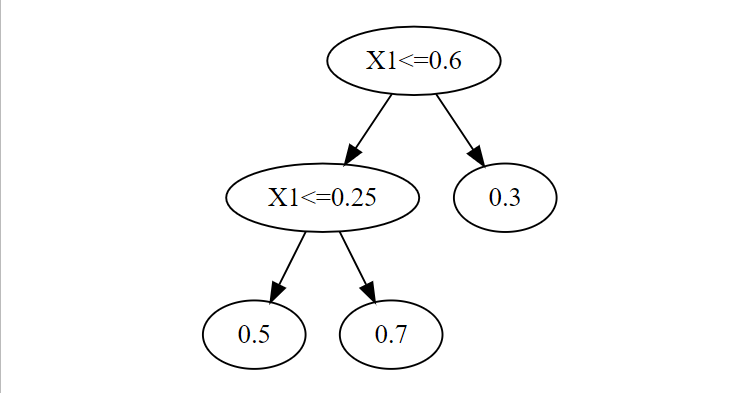
\includegraphics[width=0.5\linewidth]{tree_cond_tau_x.png}
\end{figure}

\begin{figure}
	\centering
	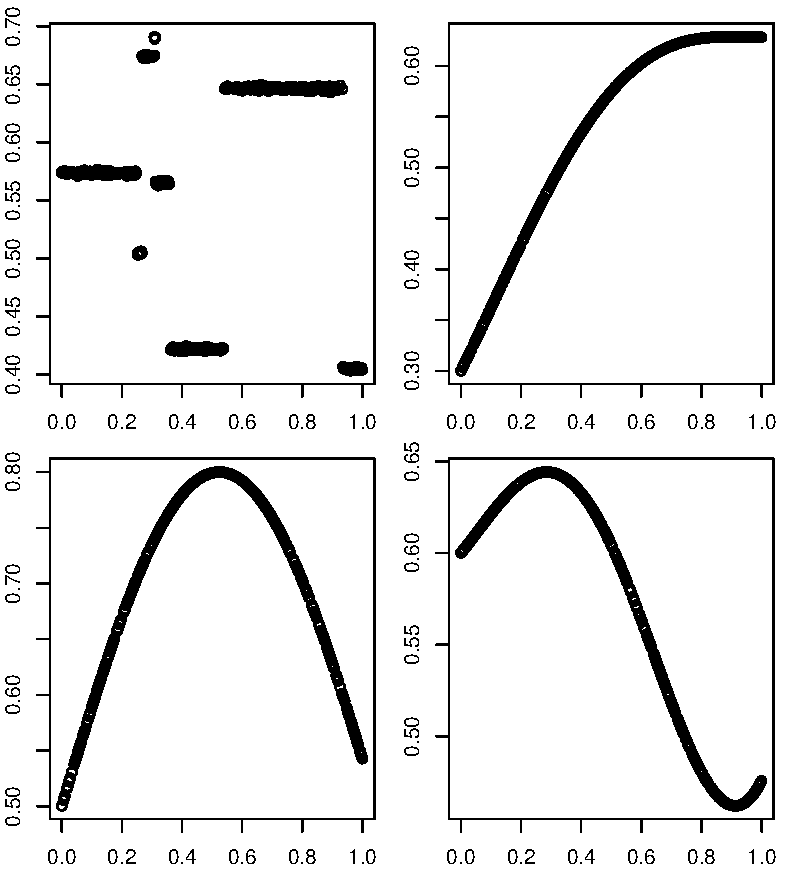
\includegraphics[width=0.95\linewidth]{true_tau.pdf}
	\caption{True values of Kendall's $\tau$ with respect to $x$. The top left plot shows case with tree structure; top right plot shows case defined by \cref{eq:synth:tau_x:case2}; bottom left shows case defined by \cref{eq:synth:tau_x:case3}; and bottom right shows case defined by \cref{eq:synth:tau_x:case4}.}
	\label{fig:true:tau}
\end{figure}

Then using these values of conditional Kendall's $\tau$, we generate the copula parameters using the link functions summarised in \cref{tab:cop:link}. Afterwards, we simulate from the copula density functions to obtain our synthetic dataset.

\begin{table}
	\centering
	\begin{tabular}{l|c|c|c}
		\toprule
		Family & Support & Relation with $\tau$ & Range of $\tau$ \\
		\midrule
		Gaussian & $\rho \in (-1,1)$ & $\sin(\tau\pi/2)$ & (-1,1)\\
		Student-t & $\rho \in (-1,1)$ & $\sin(\tau\pi/2)$ & (-1,1) \\
		Clayton & $\theta \in (0,\infty)$ & $2\tau/(1-\tau)$ & $(0,1)$ \\
		Gumbel & $\theta\in [1,\infty)$ & $1/(1-\tau)$  & $[0,1)$ \\
		\bottomrule
	\end{tabular}
	\caption{Copula families used for analyses, along with parameter support and relation with Kendall's $\tau$.}
	\label{tab:cop:link}
\end{table}

\paragraph{Prediction accuracy} For the sake of evaluating the efficiency of copula parameter estimation we check in sample prediction of the copula parameter ($\rho$ for Gaussian and student-t; $\theta$ for Clayton and Gumbel) using the posterior samples of the regression trees . 

There after we check the root mean squared error with respect to the true copula parameter used in the data generation phase. Given by:

\begin{equation}
	\text{RMSE} = \sqrt{\frac{1}{nC}\sum_{j=1}^C \sum_{i=1}^n (\theta_{ij} - \overline{\theta}^*_{ij})^2}
\end{equation}
where $\overline{\theta}^*_i$ is posterior sample mean of copula parameter conditional on $x_i$ and $C$ is the total number of parallel chains.

For accuracy, we check whether the true copula parameter is contained within the 95\% credible interval of the predictive samples of the copula parameter

\begin{equation}
	\text{Accuracy} = \frac{\sum_{j=1}^C\sum_{i=1}^n\mathbb{I}\left(Q_{2.5}(\theta^*_{ij}) \le \theta_i \le Q_{97.5}(\theta^*_{ij})\right)}{nC}.
\end{equation}

Additionally, we check for credible interval length using $\left(Q_{97.5}(\theta^*_i) - Q_{2.5}(\theta^*_i)\right)$.

\paragraph{Results}

We present the summary of our analyses with different copulas in \cref{tab:gauss:summary} and convergence diagnostics in \cref{tab:gauss:convergence}.

\begin{table}[ht]
	\centering
	\scriptsize{
	\begin{tabular}{lc|cccccc}
		\toprule
		Case & Trees & $\mathbb{E}(n_L\mid U,X)$ & $\mathbb{E}(D\mid U,X)$ & Acc. Rate & RMSE & CI length & Accuracy \\ 
		\midrule
		\multicolumn{8}{c}{Gaussian} \\
		\midrule
		Case 1 & 1 & 3.0870 & 1.9988 & 0.4245 & 0.0031 & 0.1879 & 0.8520 \\ 
		Case 1 & 5 & 2.2083 & 1.1993 & 0.2405 & 0.0042 & 0.2568 & 0.9020 \\ 
		Case 2 & 1 & 2.1405 & 1.1378 & 0.1185 & 0.0069 & 0.1278 & 0.5020 \\ 
		Case 2 & 5 & 2.1980 & 1.1911 & 0.2875 & 0.0045 & 0.2232 & 0.9580 \\ 
		Case 3 & 1 & 2.9807 & 1.9513 & 0.4065 & 0.0014 & 0.0860 & 0.6540 \\
		Case 3 & 5 & 2.2292 & 1.2097 & 0.2627 & 0.0009 & 0.1235 & 0.8760 \\ 
		Case 4 & 1 & 2.0493 & 1.0480 & 0.0873 & 0.0017 & 0.1126 & 0.8520 \\ 
		Case 4 & 5 & 2.2187 & 1.2044 & 0.3144 & 0.0019 & 0.2002 & 0.9440 \\ 
		\midrule
		\multicolumn{8}{c}{Student t} \\
		\midrule
		Case 1 & 1 & 3.0792 & 2.0195 & 0.4302 & 0.0017 & 0.1412 & 0.9440 \\ 
		Case 1 & 5 & 3.0792 & 2.0195 & 0.4302 & 0.0017 & 0.1412 & 0.9440 \\ 
		Case 2 & 1 & 2.3683 & 1.3438 & 0.2757 & 0.0018 & 0.2140 & \textbf{0.6800} \\ 
		Case 2 & 5 & -- & -- & 0.3321 & 0.0055 & 0.2424 & 0.9420 \\
		Case 3 & 1 & 3.1178 & 2.0320 & 0.4413 & 0.0074 & 0.1023 & \textbf{0.4000} \\ 
		Case 3 & 5 & -- & -- & 0.3165 & 0.0032 & 0.1308 & 0.8860 \\
		Case 4 & 1 & 2.0758 & 1.0685 & 0.2165 & 0.0009 & 0.1172 & 0.9680 \\ 
		Case 4 & 5 & 2.0758 & 1.0685 & 0.2165 & 0.0009 & 0.1172 & 0.9680 \\ 
		\midrule
		\multicolumn{8}{c}{Clayton} \\
		\midrule
		Case 1 & 1 & 3.0160 & 2.0095 & 0.4128 & 0.0220 & 0.7504 & 1.0000 \\ 
		Case 1 & 5 & 3.0160 & 2.0095 & 0.4128 & 0.0220 & 0.7504 & 1.0000 \\ 
		Case 2 & 1 & 2.0278 & 1.0278 & 0.0472 & 0.1862 & 0.8522 & \textbf{0.7420} \\ 
		Case 2 & 5 & 2.0278 & 1.0278 & 0.0472 & 0.1862 & 0.8522 & \textbf{0.7420} \\ 
		Case 3 & 1 & 2.8338 & 1.7613 & 0.3493 & 1.1694 & 2.5060 & \textbf{0.6620} \\ 
		Case 3 & 5 & 2.8338 & 1.7613 & 0.3493 & 1.1694 & 2.5060 & \textbf{0.6620} \\ 
		Case 4 & 1 & 2.0277 & 1.0277 & 0.1670 & 0.1396 & 0.9837 & \textbf{0.6920} \\
		Case 4 & 5 & 2.0277 & 1.0277 & 0.1670 & 0.1396 & 0.9837 & \textbf{0.6920} \\
		\midrule
		\multicolumn{8}{c}{Gumbel} \\
		\midrule
		Case 1 & 1 & 2.1182 & 1.1173 & 0.0915 & 0.2654 & 0.5034 & \textbf{0.3980} \\ 
		Case 1 & 5 & -- & -- & 0.2648 & 0.1148 & 0.8510 & 0.8780 \\
		Case 2 & 1 & 2.1218 & 1.1198 & 0.1262 & 0.0427 & 0.8122 & 0.9300 \\ 
		Case 2 & 5 & 2.1218 & 1.1198 & 0.1262 & 0.0427 & 0.8122 & 0.9300 \\ 
		Case 3 & 1 & 3.1997 & 2.0167 & 0.4438 & 0.1313 & 1.2414 & \textbf{0.8120} \\ 
		Case 3 & 5 & -- & -- & 0.2643 & 0.0607 & 1.4935 & 0.9860 \\
		Case 4 & 1 & 2.0287 & 1.0287 & 0.1182 & 0.0492 & 0.5881 & \textbf{0.6920} \\ 
		Case 4 & 5 & 2.0287 & 1.0287 & 0.1182 & 0.0492 & 0.5881 & \textbf{0.6920} \\ 
		\bottomrule
		\end{tabular}}
	\caption{Summary of analyses with Gaussian copula. The columns represents the specific case, the type of prior on $\mu_j\mid T$, the posterior expected number of terminal nodes, the posterior expected depth, the acceptance rate of MH algorithm, RMSE of estimated $\rho$ against true $\rho$, length of credible interval and coverage frequency within the credible interval. The posterior quantities are obtained by running 100 different chains with 6000 samples in a single chain. We discard 1000 samples and then it is thinned by 10.}
	\label{tab:gauss:summary}
\end{table}


\begin{table}[ht]
	\centering
	\scriptsize{
		\begin{tabular}{lc|crr|crr|crr}
			\toprule
			\multicolumn{2}{c|}{} &
			\multicolumn{3}{c|}{Depth} &
			\multicolumn{3}{c|}{$n_L$} &
			\multicolumn{3}{c}{likelihood} \\
			\midrule
			Case & Trees & AC & ESS (\%) & Geweke & AC & ESS (\%) & Geweke & AC & ESS (\%) & Geweke \\ 
			\midrule
			\multicolumn{11}{c}{Gaussian} \\
			\midrule
			Case 1 & 1 & 0.95 & 1.15 & 0.34 & 0.97 & 0.93 & 0.05 & 0.85 & 5.44 & 1.29 \\ 
			Case 1 & 5 & -- & -- & -- & -- & -- & -- & 0.78 & 3.92 & -1.79 \\ 
			Case 2 & 1 & 0.91 & 4.86 & 0.96 & 0.92 & 5.11 & 0.86 & 0.77 & 8.52 & 1.99 \\ 
			Case 2 & 5 & -- & -- & -- & -- & -- & -- & 0.68 & 5.89 & 0.68 \\ 
			Case 3 & 1 & 0.91 & 7.47 &  & 0.93 & 3.38 & -1.65 & 0.89 & 3.60 & 1.28 \\ 
			Case 3 & 5 & -- & -- & -- & -- & -- & -- & 0.75 & 3.90 & 0.35 \\ 
			Case 4 & 1 & 0.93 & 2.77 & 1.24 & 0.93 & 2.44 & 1.24 & 0.84 & 6.52 & 1.86 \\ 
			Case 4 & 5 & -- & -- & -- & -- & -- & -- & 0.74 & 3.23 & 3.25 \\ 
			\midrule
			\multicolumn{11}{c}{Student t} \\
			\midrule
			Case 1 & 1 & 0.35 & 54.36 & 0.42 & 0.51 & 40.22 & 0.65 & 0.08 & 60.79 & 1.24 \\ 
			Case 1 & 5 & 0.35 & 54.36 & 0.42 & 0.51 & 40.22 & 0.65 & 0.08 & 60.79 & 1.24 \\ 
			Case 2 & 1 & 0.43 & 39.64 & -0.33 & 0.48 & 34.93 & -0.41 & 0.38 & 33.58 & 0.77 \\ 
			Case 3 & 1 & 0.39 & 51.65 & -2.57 & 0.58 & 29.10 & -0.49 & 0.11 & 17.62 & -0.77 \\ 
			Case 4 & 1 & 0.50 & 24.27 & -0.44 & 0.51 & 25.01 & -0.44 & -0.02 & 100.00 & 0.82 \\ 
			\midrule
			\multicolumn{11}{c}{Clayton} \\
			\midrule
			Case 1 & 1 & 0.33 & 65.06 & -1.07 & 0.33 & 66.13 & 0.79 & 0.08 & 74.75 & -1.36 \\ 
			Case 1 & 5 & 0.33 & 65.06 & -1.07 & 0.33 & 66.13 & 0.79 & 0.08 & 74.75 & -1.36 \\ 
			Case 2 & 1 & 0.34 & 56.56 & -2.35 & 0.34 & 56.56 & -2.35 & 0.28 & 36.34 & -1.58 \\ 
			Case 2 & 5 & 0.34 & 56.56 & -2.35 & 0.34 & 56.56 & -2.35 & 0.28 & 36.34 & -1.58 \\ 
			Case 3 & 1 & 0.53 & 5.79 & -0.78 & 0.57 & 18.35 & -0.85 & 0.28 & 39.57 & -0.85 \\ 
			Case 3 & 5 & 0.53 & 5.79 & -0.78 & 0.57 & 18.35 & -0.85 & 0.28 & 39.57 & -0.85 \\ 
			Case 4 & 1 & 0.26 & 71.26 & -2.28 & 0.26 & 71.26 & -2.28 & 0.09 & 82.51 & -0.91 \\ 
			Case 4 & 5 & 0.26 & 71.26 & -2.28 & 0.26 & 71.26 & -2.28 & 0.09 & 82.51 & -0.91 \\ 
			\midrule
			\multicolumn{11}{c}{Gumbel} \\
			\midrule
			Case 1 & 1 & 0.39 & 43.96 & -1.98 & 0.39 & 43.96 & -1.98 & 0.07 & 53.85 & 0.82 \\ 
			Case 1 & 5 & 0.39 & 43.96 & -1.98 & 0.39 & 43.96 & -1.98 & 0.07 & 53.85 & 0.82 \\ 
			Case 2 & 1 & 0.60 & 24.80 & 0.02 & 0.60 & 24.65 & 0.02 & 0.37 & 9.25 & 1.11 \\ 
			Case 2 & 5 & 0.60 & 24.80 & 0.02 & 0.60 & 24.65 & 0.02 & 0.37 & 9.25 & 1.11 \\ 
			Case 3 & 1 & 0.63 & 13.03 & -1.41 & 0.81 & 4.68 & -3.38 & 0.07 & 61.78 & 1.71 \\ 
			Case 3 & 5 & 0.63 & 13.03 & -1.41 & 0.81 & 4.68 & -3.38 & 0.07 & 61.78 & 1.71 \\ 
			Case 4 & 1 & 0.24 & 55.50 & -0.47 & 0.24 & 55.50 & -0.47 & 0.22 & 47.01 & -0.14 \\ 
			Case 4 & 5 & 0.24 & 55.50 & -0.47 & 0.24 & 55.50 & -0.47 & 0.22 & 47.01 & -0.14 \\ 
			\bottomrule
	\end{tabular}
\caption{Posterior convergence diagnostic for Different copulas. The first two columns represent the specific case, type of prior on $\mu_j\mid T$. Followed by auto-correlation (lag-1) denoted by `AC', effective sample size percentage denoted by `ESS (\%)' and Geweke score of posterior samples of depth, posterior samples of the number of terminal nodes and likelihood.}\label{tab:gauss:convergence}}
\end{table}

\appendix

\section{Derivatives}
Let $\log(f(h(\mu)))\coloneqq \log(f(h(\mu)\mid U_1,U_2,X)) = \sum\log\left(c(u_1,u_2\mid h(R_j+\mu))\right)$ denote the copula likelihood at a terminal node. Then the first derivative is given by:
\begin{align}
	\begin{split}
		\frac{\partial \log(f(h(\mu)))}{\partial \mu} 
		& = \frac{\partial f(h(\mu))}{\partial \mu}\frac{\partial \log(f(h(\mu)))}{\partial f(h(\mu))}\\
		& = \frac{\partial h(\mu)}{\partial \mu}\frac{\partial f(h(\mu))}{\partial h(\mu)}\frac{1}{f(h(\mu))} \\
		& = h'(\mu)\frac{f'(h(\mu))}{f(h(\mu))}.
	\end{split}
\end{align}

Similarly, the second derivative is given by:
\begin{align}
	\begin{split}
		\frac{\partial^2 \log(f(h(\mu)))}{\partial \mu^2}
		& = \frac{\partial}{\partial \mu}\left[h'(\mu)\frac{f'(h(\mu))}{f(h(\mu))}\right]\\
		& = h''(\mu)\frac{f'(h(\mu))}{f(h(\mu))} 
			+ h'(\mu)\frac{\partial}{\partial \mu}\left[\frac{f'(h(\mu))}{f(h(\mu))}\right]\\
		& = h''(\mu)\frac{f'(h(\mu))}{f(h(\mu))} 
		+ \left(h'(\mu)\right)^2\left[\frac{f''(h(\mu))}{f(h(\mu))} - \left(\frac{f'(h(\mu))}{f(h(\mu))}\right)^2\right]
	\end{split}
\end{align}

\bibliographystyle{plainnat}
\bibliography{example}

\end{document}
